%\subsection{Histogramm f\"ur Threats to Validity (167)}
%\begin{figure}
\begin{center}
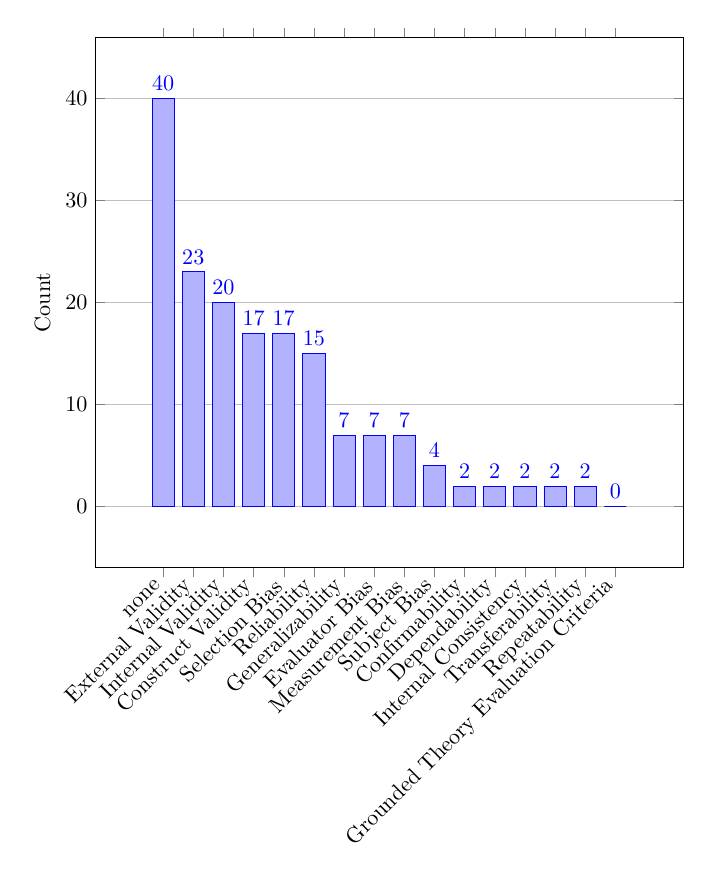
\begin{tikzpicture}[scale=.8]
\begin{axis}[ ybar, ymajorgrids, enlargelimits=0.15, legend style={at={(0.5,-0.15)}, anchor=north,legend columns=-1},
    width=.90\linewidth,height=10cm,
    nodes near coords, %nodes near coords align=below,
    ylabel={Count}, ymin=0,
    x tick label style={rotate=45,anchor=east},
    xtick={1,2,3,4,5,6,7,8,9,10,11,12,13,14,15,16},
    xticklabels={none, External Validity, Internal Validity, Construct Validity, Selection Bias, Reliability, Generalizability, Evaluator Bias, Measurement Bias, Subject Bias, Confirmability, Dependability, Internal Consistency ,Transferability, Repeatability, Grounded Theory Evaluation Criteria
}
    %xlabel={Threats to Validity}    
    ]
  \addplot coordinates { (1,40)  (2,23)  (3,20)  (4,17)  (5,17)  (6,15)  (7,7)  (8,7)  (9,7)  (10,4)  (11,2)  (12,2)  (13,2)  (14,2)  (15,2)  (16,0)   };
\end{axis}
\end{tikzpicture}
\end{center}
%\caption{Histogramm f\"ur Threats to Validity (167)}
%\label{fig:histo_threatstovalidity}
%\end{figure}

